\clearpage
\begin{usecase}
  \addheading{Use-Case Description}
  \addsingletwocolumnrow{Name}{suDeployAndRun}
  \addsingletwocolumnrow{Scope}{System}
  \addsingletwocolumnrow{Altitude}{Summary}
  
  \addrowheading{Parameters}
  \addnumberedsinglerow{}{none}

  \addrowheading{Primary actor(s)}
  \addnumberedsinglerow{}{\msrcode{actAdministrator[active]}}
  
  \addrowheading{Secondary actor(s)}
  \addnumberedsinglerow{}{\msrcode{actMsrCreator[active]}}
  \addnumberedsinglerow{}{\msrcode{actCoordinator[active]}}
  \addnumberedsinglerow{}{\msrcode{actComCompany[active]}}
  
  \addrowheading{Goal(s) description}
  \addsinglerow{The goal is to install the \msricrash system on its infrastructure and to exploit its capacities related to the secure administration and efficient handling of car crash crisis situations depending on alerts received.}
  
  \addrowheading{Reuse}
  \addnumberedsinglerow{}{\msrucname{oeCreateSystemAndEnvironment}}
  \addnumberedsinglerow{}{\msrucname{ugAdministrateTheSystem}[1..*]}
  \addnumberedsinglerow{}{\msrucname{suGlobalCrisisHandling}[1..*]}
  \addnumberedsinglerow{}{\msrucname{oeAlert}[1..*]}
  
  \addrowheading{Protocol condition(s)}
  \addnumberedsinglerow{}{the \msricrash system has never been deployed and used}
  
  \addrowheading{Pre-condition(s)}
  \addnumberedsinglerow{}{none}
  
  \addrowheading{Main post-condition(s)}
  \addnumberedsinglerow{}{\msricrash system has been created and able to handled
  the crisis situations for which it received alerts through the communication company.}
  
  
  \addrowheading{Main success steps}
  \addalphanumberedsinglerow{}{the actor \msrcode{actMsrCreator} executes the \msrucname{oeCreateSystemAndEnvironment} use case}
  \addalphanumberedsinglerow{}{the actor \msrcode{actAdministrator} executes the \msrucname{ugAdministrateTheSystem} use case}
  \addalphanumberedsinglerow{}{the actor \msrcode{actComCompany} executes the \msrucname{oeAlert} use case}
  \addalphanumberedsinglerow{}{the actor \msrcode{actCoordinator} executes the \msrucname{suGlobalCrisisHandling} use case}
  
  \addrowheading{Step Constraints Ordering and Extensions}
  \addnumberedsinglerow{}{step (a) must be always the first step.}
  \addnumberedsinglerow{}{step (b) (c) and (d) executions are interleaved.}
  \addnumberedsinglerow{}{step (b) (c) (d) can be executed multiple times.}
  \addnumberedsinglerow{}{step (d) can be executed by different
  \msrcode{actCoordinator} actors.}
  \addnumberedsinglerow{}{step (d) can be executed as a reaction to step (c).}
  
  \addrowheading{Additional Information}
  \addsinglerow{none}
\end{usecase} 

 \clearpage

 \clearpage

 \begin{figure}[htbp]
 \begin{center} 
 \scalebox{0.95}{
 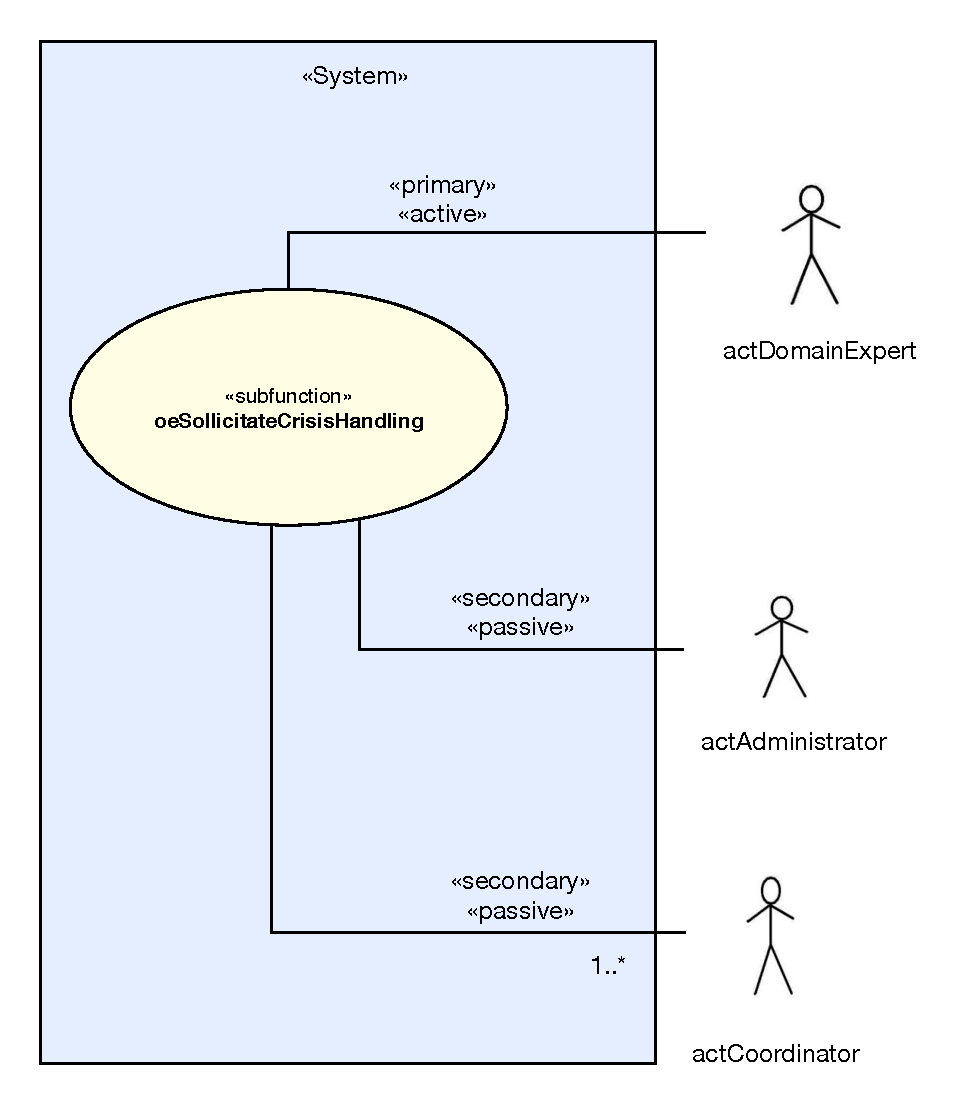
\includegraphics[width=180mm]{./images/oeDeployAndRun.eps}
 \normalsize}
 \end{center}
 \caption[\msricrash Use Case Diagram:  oeDeployAndRun Diagram]{\msricrash Use Case Diagram:  oeDeployAndRun}
 \label{fig:icrash-RE-UCD- oeDeployAndRun}
 \end{figure}
 \vspace{0.5cm}
